\chapter{Conclusiones}
En este capítulo se presenta el análisis de los resultados obtenidos, las limitaciones encontradas y algunas consideraciones y mejoras para trabajos futuros.

\section{Casos especiales}
Existen algunos casos para los cuales el algoritmo no proporciona un rendimiento adecuado, los cuales se describen a continuación.

\subsection{Iluminación excesiva}
Una iluminación excesiva (\Cref{img:light_1_rgb}) puede crear matices falsos en el canal Hue (\Cref{img:light_1_hue}) lo cual provocará una segmentación incorrecta de la imagen (\Cref{img:light_1_binary}).

\begin{figure}[H]
\centering
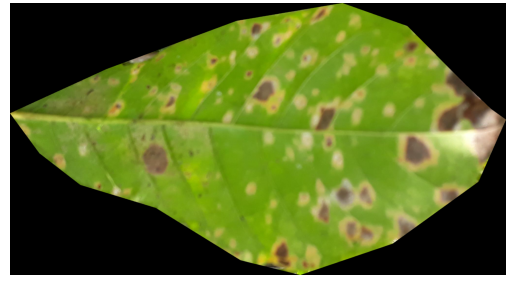
\includegraphics[scale=1]{images/special_case_light_1_rgb.png}
\caption{Iluminación excesiva en una hoja}
\label{img:light_1_rgb}
\end{figure}

\begin{figure}[H]
\centering
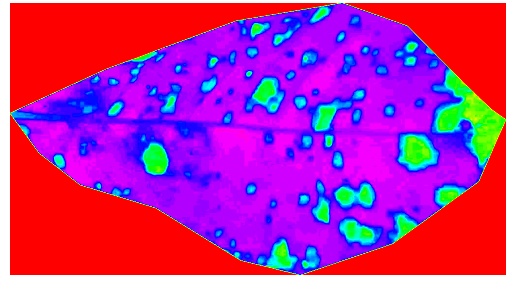
\includegraphics[scale=1]{images/special_case_light_1_hue.png}
\caption{Matices falsos por iluminación excesiva}
\label{img:light_1_hue}
\end{figure}

\begin{figure}[H]
\centering
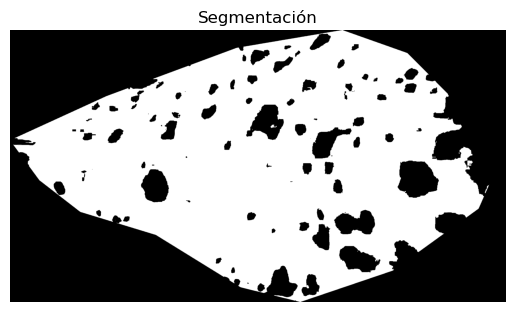
\includegraphics[scale=1]{images/special_case_light_1_binary.png}
\caption{Segmentación de una hoja con iluminación excesiva}
\label{img:light_1_binary}
\end{figure}

\subsection{Iluminación artificial o no contemplada}
De igual manera, una iluminación creada por una fuente artificial (una lámpara) o no contemplada (día nublado), puede causar un despliegue de la imagen inconsistente o contraintuitivo (\Cref{img:light_2_hue}).

\begin{figure}[H]
\centering
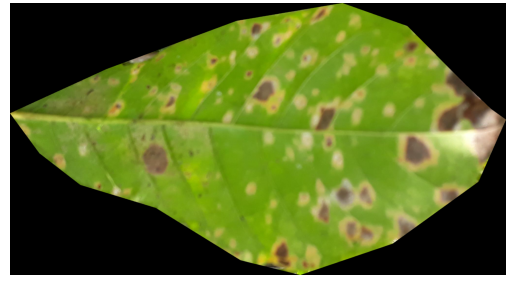
\includegraphics[scale=1]{images/special_case_light_2_rgb.png}
\caption{Hoja con iluminación no contemplada}
\label{img:light_2_rgb}
\end{figure}

\begin{figure}[H]
\centering
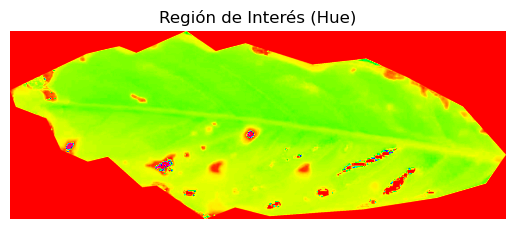
\includegraphics[scale=1]{images/special_case_light_2_hue.png}
\caption{Despliegue contraintuitivo de una imagen}
\label{img:light_2_hue}
\end{figure}

\begin{figure}[H]
\centering
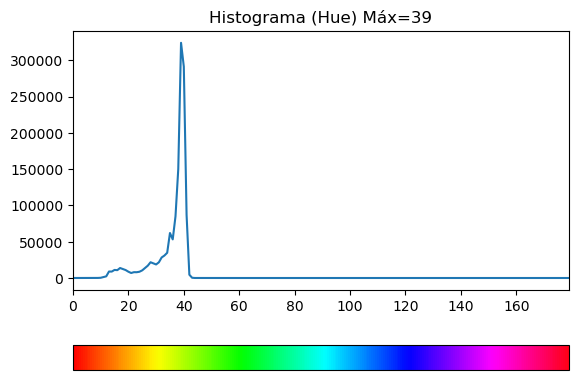
\includegraphics[width=\textwidth]{images/special_case_light_2_histogram.png}
\caption{Histograma de una imagen con despliegue contraintuitivo}
\label{img:light_2_binary}
\end{figure}

\subsection{Envés de la hoja}
El algoritmo ignora el haz y el envés (\Cref{img:backbone_rgb}) de la hoja, por lo tanto, aplica el mismo proceso en ambas condiciones. Sin embargo, los nervios de la hoja presentan, generalmente, un matiz diferente al resto de la hoja (\Cref{img:backbone_hue}), provocando que la segmentación sea errónea (\Cref{img:backbone_binary}).

\begin{figure}[H]
\centering
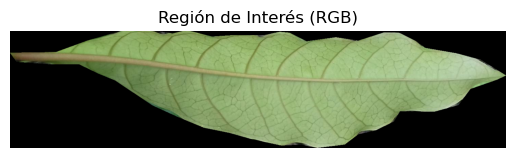
\includegraphics[scale=1]{images/special_case_backbone_rgb.png}
\caption{Envés de una hoja saludable}
\label{img:backbone_rgb}
\end{figure}

\begin{figure}[H]
\centering
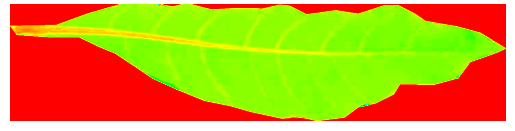
\includegraphics[scale=1]{images/special_case_backbone_hue.png}
\caption{Canal Hue del envés de una hoja saludable}
\label{img:backbone_hue}
\end{figure}

\begin{figure}[H]
\centering

\includegraphics[scale=1]{images/special_case_backbone_binary.png}
\caption{Segmentación del envés de una hoja saludable}
\label{img:backbone_binary}
\end{figure}

\section{Conclusiones específicas}

\section{Conclusiones generales}

\section{Mejoras y trabajo a futuro}